


% Notes on style
%
% Identation
% Variable names
% Magic numbers, introducing final
%
% git commit file
%
% Reciprocal of Integer.parseInt() -> String.valueOf(int)
%
%
% PART-TIMERS
% Day 2: create account on GitHub like bbk-pij-2012-XX
%        for loops
%
%
% Java Decaf should have arrays


\section{Introduction}
\label{sec:introduction}

Programs have lots of data, they are basically
ways of getting data, transforming data, and giving data back to the
world. 
%
Data types, as we have already seen, tell you which kinds of data you
have in your program. 

Computers store data in their memory in the form of bits. The word
``bit'' is a contraction of ``BInary digiT'', so a bit is
either~1~or~0, true or false, high or low, on or off. Bits are
organised in groups of 8 called \emph{bytes}. These bytes ---groups of
eight bits--- are used to store any data in the memory of the
computer. When you have got~1024~bytes, you have got a kilobyte or kB;
when you have~1024~kB you have got a megabyte or MB, and so on for
gigabytes~(GB), terabytes~(TB), and petabytes~(PB). Note that in
computing everything is measured in powers of~2 ($2^3 = 8, 2^{10} =
1024$) and not in powers of~10 as in normal life. That is because
computers count with bits~(2) and human beings\footnote{Not all humans
used only the ten fingers in their hands to count. Some languages like
French or Irish have remains of base-20 counting.} count with their
fingers~(10). 

\section{Simple data types}
\label{sec:simple-data-types}

Simple data types can be thought as boxes in the computer's
memory. Every time you declare a variable in your program, you can
think\footnote{This is only a metaphore and is not supposed to be an
  accurate description of how memory is managed on a modern
  computer. Explaining how things like the registers, the stack, and
  the heap work, the differences between actual machines and virtual
  machines, etc; are out of the scope of this document.} of the
computer as creating a little box in its memory to store your
variable. That box has two tags on it: one of them holds the name of
the variable and the other holds the type
(Figure~\ref{fig:github}). In the same way, you can think of
assignment as putting a value inside that box. 

\begin{figure}
  \centering
  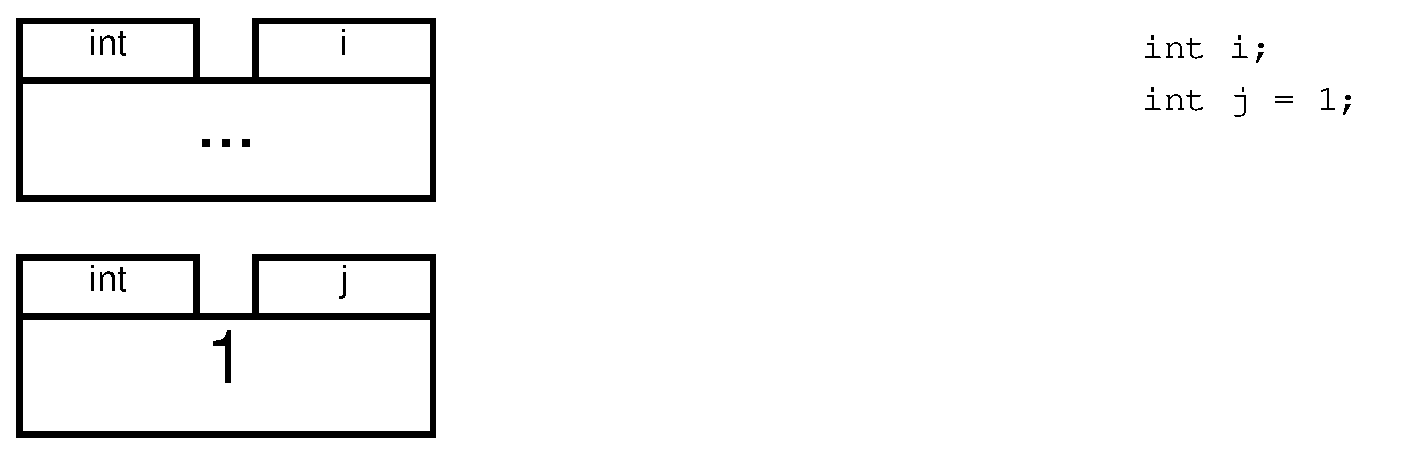
\includegraphics[width=\textwidth]{gfx/variables1}
  \caption{Declaring a variable in Groovy can be seen as creating a
    box. The box has a tag for the name and another for the type.}
  \label{fig:var1}
\end{figure}

\begin{figure}
  \centering
  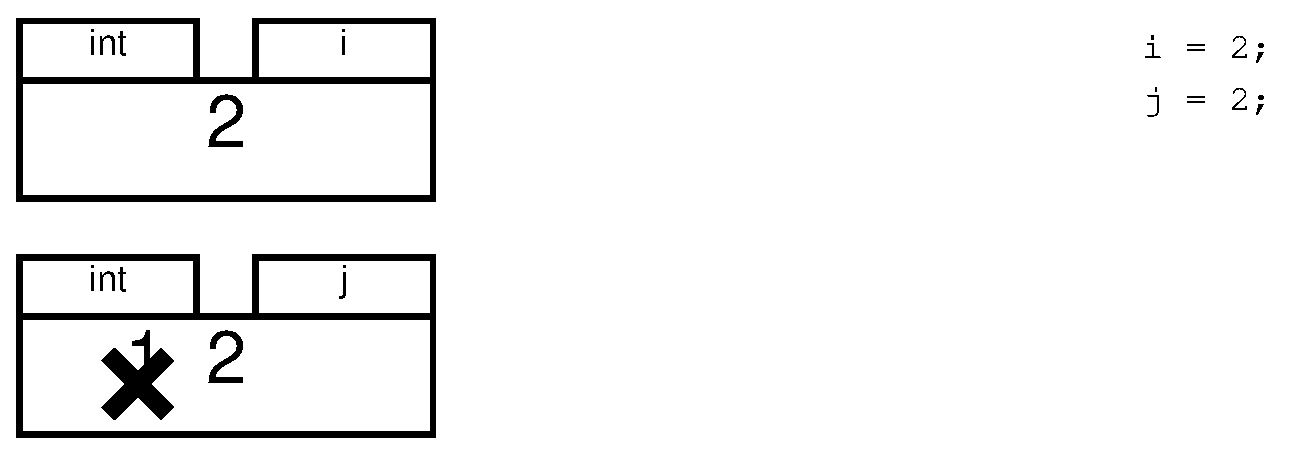
\includegraphics[width=\textwidth]{gfx/variables2}
  \caption{Assigning a value to a variable can be seen as putting a
    value in the box. If there was something in the box, it is
    overwritten and lost forever.}
  \label{fig:var2}
\end{figure}

\subsection{Static typing and dynamic typing}
\label{sec:strong-typing-weak}

You have already seen that Groovy, as most languages, puts some
restrictions to what you can use as a ``name'' tag for your boxes. You
know that they have to start with a letter: ``count'' is a valid name
but ``/me'' or ``5thNumber'' are not. You also know that some words
cannot be used by the programmer for variables names because it would
be confusing, e.g. ``while'', ``if'', ``System'', or ``println''.

Many programming languages also place one restriction on the ``type''
tag: once you decide the type of a variable, you cannot change
it. This is like people having static opinions that they do not want
to change. This type of languages are called \emph{statically typed
  languages} and, contrary to people with fixed ideas, they are
not necessarily bad or obnoxious. Java is an example of
statically typed language. 

Some programming languages allow you to change the type of your
variables as you go along, so you can have a variable that sometimes
is an int and later in time is a boolean or a String. These languages
are called \emph{dynamically typed languages}. They have pros and cons
compared to their statically typed counterparts. Groovy is an example
of a dynamically typed language. The following code excerpt is valid
in Groovy but not in Java. In Java a variable cannot be a String, and
then a boolean, and then a String again. Note that \emph{true} is a
boolean while \emph{``true''} (in quotes) is a String. 

\begin{verbatim}
    String str = "This is a string";
    str = true;   // This is different to: str = "true"
    if (str) {
      str = "This is a different string";
    }
\end{verbatim}

There are many more things to know about typing in programming
languages (strong vs. weak, inferred vs. manifest, duck typing, and
much more) but for now it will not be necessary to go into those
details. 

\subsection{Most common simple types}
\label{sec:most-common-simple}

\subsubsection{Integer numbers}
\label{sec:integers}

Integers (\verb+int+) are probably the most used simple data type, as
integer numbers are used for two of the most common operations in
computing: counting and indexing. Integers use~32~bits of memory, and
an integer variable can hold values between~-2,147,483,648 and
2,147,483,647~(inclusive). This data type is large enough for the
numbers needed in~90\%~of programs most people write. We have already
seen how to use it: 

\begin{verbatim}
    int count = 1
\end{verbatim}

There are two versions of integers for some special uses. When a
program needs very large (positive or negative) values, there is a
type \verb+long+, for \emph{long integer}. It is called ``long''
because it uses 64~bits instead of 32, which means a long integer
variable can hold values between -9,223,372,036,854,775,808 and
9,223,372,036,854,775,807 (inclusive). There is also a ``short''
integer that uses only 16~bits of memory (\verb+short+); this was
sometimes useful when Java was first released in 1995 but is hardly
ever used with modern computers. 

\subsubsection{Floating-point (decimal/rational) numbers}
\label{sec:float-point-decim}

Not all numbers are integer. Examples of common non-integer numbers
include the result of a division of two integers where one is not a
multiple of the other, and real-measurements like your height, your
weight, and the distance between your workplace and your home (unless
you work at home). In maths, these are called real numbers. In
computing they are usually called floating-point numbers and are
represented as a list of significant numbers and an exponent. The term
``floating-point'' refers to the fact that the decimal point can "float",
that is, it can be placed anywhere in the number changing the exponent
accordingly. 

$$ 1.23 \cdot 10^{-3} = 123 \cdot 10^{-5} = 0.00123 \cdot 10^0 $$

In Groovy and in Java, real numbers are usually represented with the
simple data type \verb+double+, that uses 64~bits. There is also a
32-bit version called \verb+float+ but, as with \verb+short+, it is
hardly used today.

\paragraph{Important note.} 

Floating-point numbers do \emph{not} have infinite precision, and
operating with them can cause rounding errors. There is a special type
for representing real values where precision is paramount (like in
banking): \verb+BigDecimal+. 

\subsubsection{Boolean (binary) values}
\label{sec:bool-binary-valu}

This simple data type represents one bit of information. It can hold
the values \verb+true+ and \verb+false+. 

\subsubsection{Characters}
\label{sec:characters}

Text is composed of characters: 'a', 'b', 'c'\ldots The \verb+char+ is
used to represent characters. It uses 16~bits, meaning it can
represent any of~65,536~different characters. 

Actually, the 16~bits of a char represent a Unicode symbol. Unicode is
a computing industry standard for the consistent encoding,
representation and handling of text expressed in most of the world's
writing systems. It includes symbols from most writing systems in
the world, including alphabets like Latin, Cyrillic, Arabic, or
Hebrew; syllabaries like Japanese katakana and hiragana, or
Cherokee; and many more. 

You may have noticed that we have not mentioned String yet. This is
because String is a complex type. 

\section{Complex types}
\label{sec:complex-types}

Complex types are types of data that do not fit in a box, not even in
one of the big 64-bit boxes used for \verb+double+. Because they do
not fit in the ``boxes'', computers have to store them somewhere
else. However, they also need to know where they are\ldots~and that is
what the boxes are used. 

Modern computers have \emph{a lot} of memory. Long forgotten are the
days when Bill Gates said: ``640kB of memory should be enough for
everything''. Part of that memory is used for the boxes (in a part of
memory called ``the stack'') and most of the rest is used for
everything else, including complex data (that part is called, quite
unceremoniously, ``the heap''). 

When your Groovy or Java code uses some complex data, the computer
stores that data in some region of the heap ---identified by a \emph{memory
  address}; then it stores the address in a box in the stack, much in
the way it stores integers and booleans. This looks similar to
Figure~\ref{fig:compledata}. The memory address in the box can be seen
as ``pointing to'' the place in memory where the real data is
stored. For this reason, we are going to call it a \emph{pointer}. 

\begin{figure}[htbp]
  \centering
  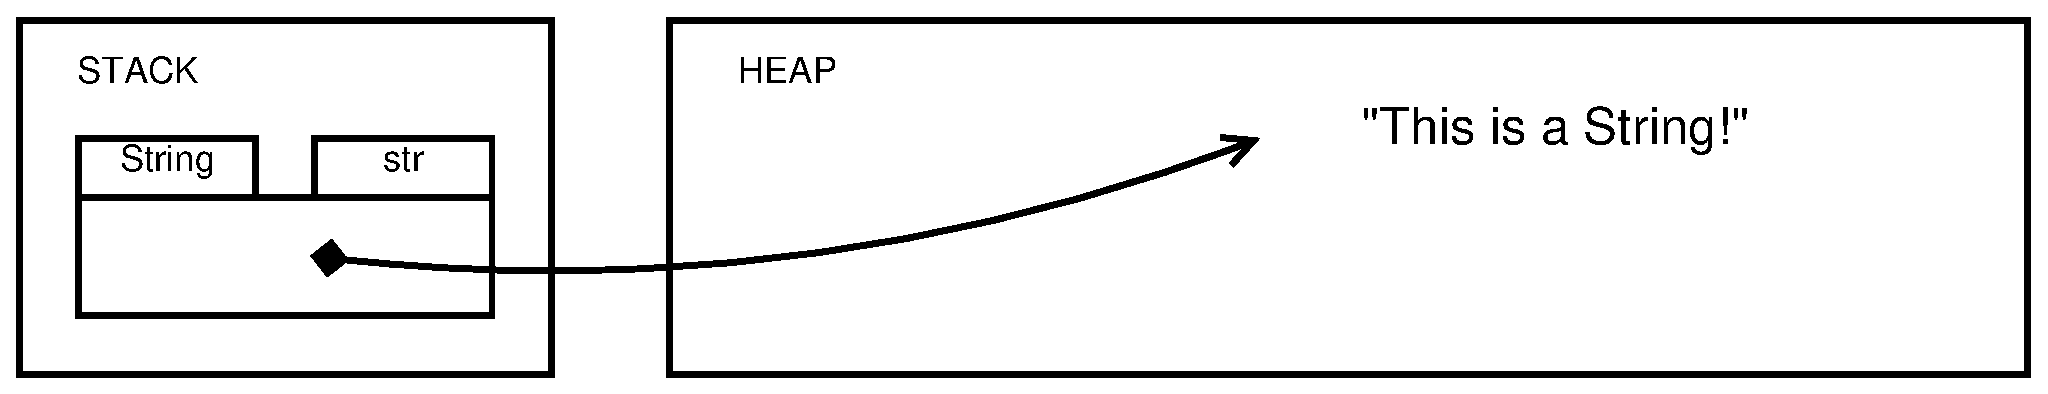
\includegraphics[width=\textwidth]{gfx/variables-string}
  \caption{A String is a type of complex data type. The data itself is
    stored in the heap and its address is stored in box in the stack
    ---pointing to it. }
  \label{fig:compledata}
\end{figure}

Using complex data types is different from using simple types in
several ways. For starters, as complex types are not stored in the
stack but in the heap, you have to \emph{allocate} memory-space in the
heap to store the data. This is done with the reserved word
\verb+new+; you also need brackets to pass arguments (as if using a
method: this is because complex types have something called a
\emph{constructor method} that we will in more detail later). We are
going to see now several examples, starting with the pervasive
Strings. 

Oh, one final note. Complex data types are usually called with capital
letters. This is not compulsory, but it is what everybody expects:
simple types with non-capital letters (e.g.~\verb+int+, \verb+double+)
and complex letters with capital letters (e.g.~\verb+String+,
\verb+Array+, \verb+List+, \verb+Customer+\ldots). If you do not
capitalise your complex types other people will get very confused when
they read your code. This is not only unpolite, it is also
unprofessional. 

\subsection{Declaration and initialisation}
\label{sec:decl-init}

When working with simple types, the memory is always used as soon as
you declare the variable. In other words, your program will use the
same amount of memory if you type \verb+int i+ and if you type
\verb+int i = 1+: it always uses 32~bits of your computer's memory. 

This is not true with complex types. When a complex type is declared
(e.g.~String str) the computer only reserves the box for the pointer,
but nothing else. It is only when the variable is \emph{allocated}
(e.g.~\verb+str = new String()+ 
or \verb+str = new String("This is a String")+) that the total amount
of memory is used. Note that the difference is huge. Boxes are 32-bit
or 64-bits long, but there is no limit to the size of a complex type:
it could be several kB or even MB (types so big are a rarity,
though). 

For any other complex type, we can make set the pointer 
not to point to any address in memory. This can be useful in
some cases that will become clearer as we learn more about
programming, including error detection and release of memory that is
no longer needed (remember that complex types can use a lot of
memory). To make a pointer point to nowhere, we use the
reserved word~\verb+null+ (with non-capital letters).

\begin{verbatim}
    String str
    str = null
\end{verbatim}

A pointer pointing to null is called a \emph{null pointer}. This
basically means that the address in the box is zero (rather than an
obscure hexadecimal number like 0x1a3ec74); the computer
knows there is never anything at address zero, so it knows a null
pointer is not being used to point to any real
data~(Figure~\ref{fig:nullpiounter}).

\begin{figure}[htbp]
  \centering
  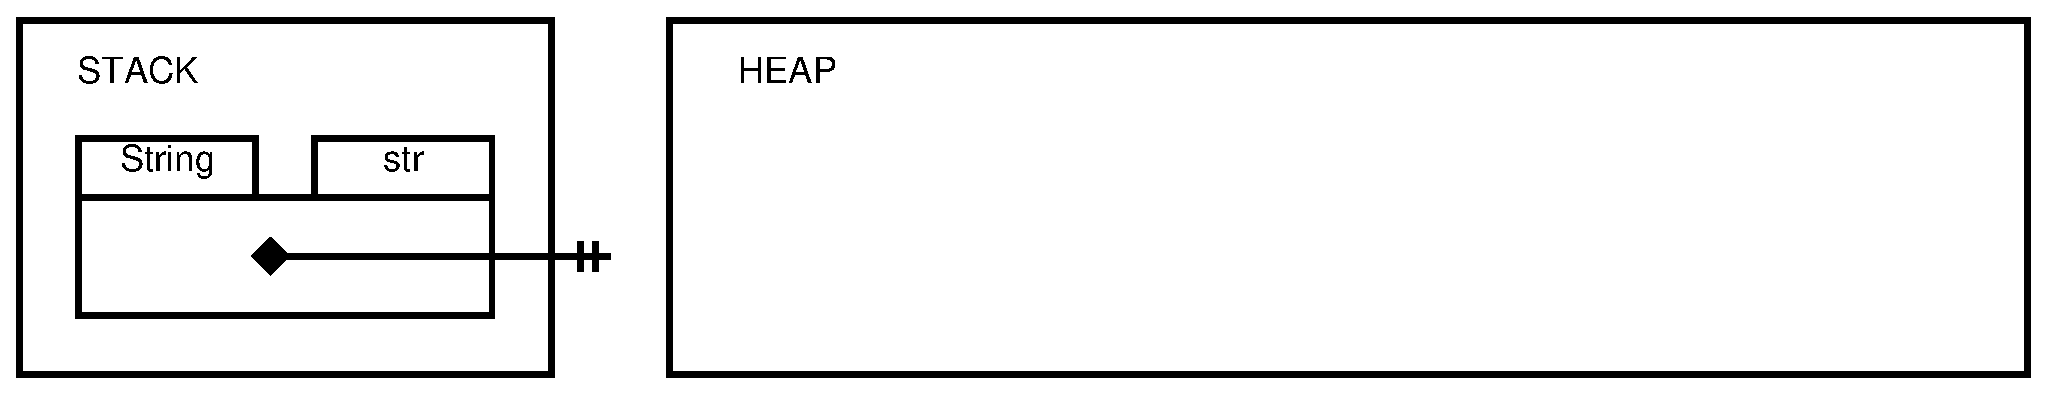
\includegraphics[width=\textwidth]{gfx/variables-string-null}
  \caption{A null pointer is basically a zero address, pointing nowhere.}
  \label{fig:nullpiounter}
\end{figure}

As a null pointer does not point to any real data, if you try to
access a variable that is pointing to null, the computer will complain
with a \verb+NullPointerException+, as in the following example: 

\begin{verbatim}
    String str = null
    println str.length()
\end{verbatim}



\subsection{String}
\label{sec:string}

Strings are everywhere. Every program, except the most trivial, uses
strings: user names, passwords, addresses, configuration options, data
input from the keyboard, a webpage read through the Wi-Fi
connection\ldots~almost anything is a String. They are the most widely
used complex types. 

At their most basic, strings are sequences of characters. You already
know how to read a piece of text from the user: 

\begin{verbatim}
   String str = System.console().readLine()
\end{verbatim}

If you want to create a string in your program without reading it from
the user, the basic form of creating a string is like this: 

\begin{verbatim}
    String str = new String("This is a String")
\end{verbatim}

but you already know that this can be made in an easier way: 

\begin{verbatim}
    String str = "This is a String"
\end{verbatim}

The former two statements are equivalent in Groovy\footnote{They are
  NOT equivalent in Java, but we will learn why when the time
  comes.}, only the second is more convenient and most people use it
instead of the other. 

It is important to note that a String with only one characters is
still one string. Strings are enclosed in double quotes, while
characters are enclosed in simple quotes:

\begin{verbatim}
   char oneChar = 'a'
   String oneCharString = "a"
\end{verbatim}

% Simple proof of non-equivalence in Java:
% 
% public class StringTest {
%    public static void main(String args[]) {
% 	 String s1 = System.console().readLine();
% 	 String s2 = new String("QWE");
% 	 String s3 = "QWE";
% 	 if (s1 == s2) System.out.println( "s1 == s2");
% 	 if (s2 == s3) System.out.println( "s2 == s3");
% 	 if (s3 == s1) System.out.println( "s3 == s1");
%    }
% }

You already know that you can do some things with strings using
\emph{methods}. Although we are going to learn more about methods on
the next section, we can introduce some of them now to help with the
exercises. Assuming you have a String called \verb+str+, you can use
the following methods:

\begin{description}
\item[str.length(): ] this method returns the length of the string.
\item[str.charAt(): ] this method requires an integer inside the
  brackets, and returns the character at the specified position;
  note that the first character is at position 0, not 1.
\item[str.substring(): ] this method requires two integers inside the
  brackets, separated by a comma, and returns another string that
  begins at the character specified by the first number and extends to
  the character specified by the second number minus one\footnote{This
  results in the substring having a length of
  secondNumber~-~firstNumber.}.  
\end{description}

Here is a brief example of how they are used. Note that if you want to
use double quotes inside double quotes, you have to \emph{escape} them
using the backslash (``\textbackslash'') sign: the backslash will make
Groovy and Java treat the next double quote as a literal double quote
and not the end of the string. 

\begin{verbatim}
    String str;
    str = new String("This is an example")
    println "Initial string: \"" + str + "\"" // Note the escaped quotes!
    int l = str.length()
    println "The length of the string is " + l
    char c = str.charAt(0)
    println "The first character is " + c
    String str2 = str.substring(8,18)
    println "The substring from char 8 to char 17 is \"" + str2 + "\""
\end{verbatim}

The result of this little program is:

\begin{verbatim}
    Initial string: "This is an example"
    The length of the string is 18
    The first ;character is T
    The substring from char 8 to char 17 is "an example"
\end{verbatim}

% \subsection{Arrays}
% \label{sec:arrays}

% A String can be seen as a series of characters one after the
% other. The idea can be extended to think of series of other simple
% types, not just chars but also integers and doubles. This is called an
% \emph{array}. 

% Arrays are a way of having several elements of data of the same type;
% for example, a company could have a payroll program with an array with
% the IDs of all its employees (an array of integers). In Groovy and
% Java, arrays can be of simple but also complex types; therefore, the
% aforementioned program could also have array of Strings to store the
% names of the employees. 

% An array is declared using square brackets. Square brackets are also
% used to access the elements in the array. Let's see an example: 

% \begin{verbatim}
%     int[] employeeIdArray;
%     employeeIdArray = new Array[5]();
%     employeeIdArray[0] = 123;
%     employeeIdArray[1] = 55;
%     employeeIdArray[2] = 14;
%     employeeIdArray[3] = 642;
%     employeeIdArray[4] = 243;
% \end{verbatim}

% As you can see, sometimes you need a number inside the brackets and
% sometimes you do not. You do need a number to declare the array,
% i.e.~to tell the computer that you want to have an array (of integers,
% in this case). As all declarations, this reserves a box of type
% ``array of integers'' and name ``employeeIdArray''. In the next line,
% we reserve a portion of memory to store the actual integers, and of
% course we have to specify the length...

% method length

% the curly bracket notation for initialisation

% You can also have arrays of arrays, in which case they are usually
% called matrices: 2-D matrices, 3-D matrices

% \subsubsection{Exercise A}
% \label{sec:exercisejfjfj}

% Write a small program that asks for the names and IDs of all employees
% in a small company, and store them in an array of integers and an
% array of Strings. The company has 10 employees.

% Use a loop to go through both arrays and print the names and IDs of
% those employees whose ID is less than 1000. Use another loop to print
% the names and IDs of those employees whose name starts with ``J''
% or~``S''. 

\subsection{You own structures: classes}
\label{sec:you-own-structures}

String is the most common complex type, but it is not the only one. As
a matter of fact, programmers can create their own type of complex
type very easily. In order to create a new type of data, we use the
keyword \verb+class+. You can think of it as creating new classes of
data. 

A new class of data must have a name (remember: by convention complex
data type start with capital letters, classes too) and be defined in
between curly brackets. A complex type is composed of several other
types, simple of complex. Let's see an example: 

\begin{verbatim}
    class Person {
      String name;
      int age;
    }
\end{verbatim}

This code defines a new class of data that represents a person, and
it is composed of a String for the name and an integer for the age. As
you can see, both simple and complex types can be used inside a
class. You can even have data on a specific class inside the same
class, as in the extended example below: 

\begin{verbatim}
    class Person {
      String name;
      int age;
      Person father;
      Person mother;
    }
\end{verbatim}

Now a person has a String for a name, an integer for the age, and two
variables of type Person for the father and the mother. Once you start
working with complex data on a regular basis (which means from now on)
you can see that it is crucial to use good identifiers for your
names. Compare the former class with this very-badly-named example: 

\begin{verbatim}
    class P {
      String s;
      int n;
      P p1;
      P p2;
    }
\end{verbatim}

Both examples contain the same information at a logical level, and the
computer will behave equally well with both. However, human
programmers reading the code will have a hell of a time trying to
understand what the second class really represents, while the first
example is obvious. Remember: source is written once but is read many
times, so your code should be as clear as possible.

Variables in a class are often called \emph{fields}. Sometimes they
are called \emph{member fields} because they can be seen as being
``part of'' (members of) the class. So the class \verb+Person+ can be
said to have four fields: one of type \verb+String+, one of type
\verb+int+, and two of type \verb+Person+. Fields in a class are
accessed using a dot, as in the following example: 

\begin{verbatim}
    Person student = new Person();
    employee.name = "John Smith";
    employee.age = 45;
    println "BOSS: How old are you, " + employee.name + "?"
    println "EMPLOYEE:  I am " + employee.age + " years old.";
\end{verbatim}

In this example we have create one piece of data of class Person, an
\emph{instance} of the class. Each of these instances of pieces of
data of a class are called \emph{objects}. Every time you use the
keyword \verb+new+ you are creating another object, and this involves
looking for a place in memory to store it and put a pointer pointing
to it. Note that fields on an object are accessed using a dot to
separate the name of the variable that identifies the object
(e.g.~employee) and the name of the variable inside the object, the
field (e.g.~name), as in \verb+employee.name+.

We can make the example slightly more complicated by using more than
one variable of the class Person. 

\begin{verbatim}
    Person john = new Person();
    john.name = "John Smith";
    john.age = 35;
    Person mary = new Person();
    mary.name = "Mary Smith";
    mary.age = 32;
    Person student = new Person();
    student.name = "John Smith, Jr.";
    student.age = 5;
    student.father = john
    student.mother = mary
    println "TEACHER: How old are you, " + student.name + "?"
    println "LITTLE JOHN: I am " + student.age + " years old, sir.";
    println "TEACHER: Who is your mother?"
    println "LITTLE JOHN: " + student.mother.name + ", sir.";
\end{verbatim}

There are two important things to learn from this example. First, we
can access data inside a complex data that itself inside another
complex data. Actually, there is no limit to the level of
encapsulation you can achieve with complex data (as long as you do not
run out of memory). If you want to access a field of a field you only
need to use two dots, as in \verb+student.mother.name+. 
Second, we
have not initialised all fields in the objects of class Person. When
you create a new object, the fields of the object have to be
initialised as any other variable, otherwise they will not have the
values you want them to have. In this example, we do not know who are
the father and the mother of objects \verb+john+ and \verb+mary+. If
we try to access them, the computer will complain. On the other hand,
if the mother of object \verb+mary+ was properly initialised, we could
know the name of the grandfather of the student by typing something
like: 

\begin{verbatim}
    println "The father of my mother is " + student.mother.father.name;
\end{verbatim}

In the next section we will see how to add methods to your classes,
like those that you know from String. 

%     int i1 = 1;
%     Integer i2 = 1;
%     if (i1 == i2) {
%       println "Nowadays you can use boxed and simple types together!";
%     }

% class E {
%   int age;
%   String name;
%   }
  
%   E e = new E()
%   e.age = 13
%   e.name = "Carlos"
%   println e.name + " tiene " + e.age + " años."
    

\subsection{Boxed types: Integer, Double, and Character}
\label{sec:boxed-types:-integer}

For every simple type in Groovy and Java, there is a ``boxed'' complex
version. The most important ones are summarised in 
Note that the name of the complex type uses capital letters and is
sometimes a longer, complete-word version of the simple type's name. 

\begin{table}[htbp]
  \centering
  \begin{tabular}{|l|l|}
    \hline
    Simple & Complex \\
    \hline
    \hline
    int & Integer \\
    double & Double \\
    char & Character \\
    \hline
  \end{tabular}
  \caption{Most importnat simple types and their boxed counterparts}
  \label{tab:jajksdfj}
\end{table}

The complex version of a simple type works mostly like any other
complex type. The variable itself contains a pointer that points to
the address in memory where the actual value is stored. Why have
complex versions of simple types? Other data types have a lot of
information (i.e. many characters in a String) and that is why they
need to be stored indirectly, but this is not the case with boxed
types. Why then? Remember that complex types of data
can have their own methods, and sometimes this is very useful. You
have come across one of the most used ones: \verb+Integer.parseInt()+,
which is used to convert strings that contain only a number into an
\verb+int+. Boxed types have several other methods, and we will see
some of them, but \verb+parseInt()+ is the one more frequently used. 

Why are these complex types called ``boxed''? This is because they can
be seen as a box wrapping around a simple type. In the old days, using
boxed types was cumbersome and boring. You could need to type
something like:

\begin{verbatim}
    int i = 1;
    Integer boxedI = new Integer(i);
    int i2 = boxedI.intValue()
\end{verbatim}

You had to explicitly create the boxed type like any other complex
type by using \verb+new+, and then you needed a method of the boxed
type to get the simple type from inside. This was a lot of work when
you had a lot of pieces of data and had to perform conversion from
simple type to boxed type very often, for example if you have to make
comparisons of data between two different sources (one simple type,
the other boxed type). This why Java (and Groovy) now
allow what is called \emph{auto-boxing}, which is just a fancy name to
say that you can use them in exactly the same way and the computer
takes care of all the boxing-in and boxing-out. In other words, the
following code is perfectly legal: 

\begin{verbatim}
    int i1 = 1
    Integer i2 = 1
    if (i1 == i2) {
      println "Nowadays you can use boxed and simple types together!"
    }
\end{verbatim}

Note that you do not need to write 
explicitly \verb+i2 = new Integer(1)+, but i2 is still a complex boxed
type, its box contains just a pointer to some place in memory where a
``1'' is stored. The variable i1, on the other hand, is a \emph{bona
  fide} integer variable, a box with a ``1'' inside. However, thanks
to auto-boxing, you can compare one with the other: the computer will
automatically extract the ``1'' inside the boxed type to perform the
comparison with the other ``1''. You do not need to do it yourself. 

\subsection{A final note on names}
\label{sec:final-note-name}

If you read other books or web pages about Groovy or Java, you may
notice that they use names that are different from the ones we have
used in this section. We go through some of them here for the sake of
clarity. 

\begin{description}
\item[Simple type: ] A type that is stored in its own box, usually
  32-bit or 64-bit long. These are usually called \emph{primitive}
  types in the Java world. I prefer to call them simple data types to
  distinguish them clearly from complex data types.
\item[Complex type: ] A type that has two parts: the box contains a
  pointer, and it points to a place in memory where the actual value
  is stored. In the Java world, these are simply called \emph{classes}
  and \emph{objects}, which is precise but fails to be explicit on the
  difference between simple and complex data types, and this can be a
  source of confusion.
\item[Pointer: ] The content of the box in a complex type, a memory
  address where actual data is stored. This is sometimes called a
  \emph{reference} or a \emph{handle} to prevent confusion with
  pointers of other languages (like C) that behave in a slightly
  different way. I think many programming languages have constructs
  that share the same name and behave in slightly different ways
  (Strings is a major example) so this is not of much
  concern. Besides, it looks to me very confusing to access a null
  ``reference'' and get a Null\emph{Pointer}Exception.
\end{description}

%%%%%%%%%%%%%%5

% Methods, functions


%%% Local Variables:
%%% mode: latex
%%% TeX-master: "main"
%%% End:

